\documentclass{article}

\usepackage[utf8]{inputenc}
\usepackage{longtable}
\usepackage{authblk}
\usepackage{adjustbox}
\usepackage{natbib}

\title{PROYECTO FINAL}
%autores
%\renewcommand\Authand{, y }
\author[1]{\normalsize Andres Felipe Cardona Rodriguez}


\affil[1]{\small  Facultad de Ingenieria Industrial, Universidad de los Andes\\
Curso: Herramientas Computacionales para la Investigacion Interdisciplinar Reproducible. IIND 4347\\}
%\texttt{{\normalsize Curso: Herramientas Computacionales para la Investigacion Interdisciplinar Reproducible. IIND 4347}}}


\affil[1]{\small Codigo: 201127229\\
Correo: af.cardona1552@uniandes.edu.co, }
%\texttt{Correos:}}

\date{01 de Julio de 2018}

\usepackage{Sweave}
\begin{document}
\Sconcordance{concordance:ProyectoFInalLatex.tex:ProyectoFInalLatex.Rnw:%
1 40 1 1 7 1 2 10 0 1 2 5 1 1 5 14 0 1 2 14 1 1 6 1 2 12 1 1 8 1 2 9 1 %
1 5 12 0 1 3 6 1 1 8 13 0 1 2 5 1 2 2 12 1 1 10 31 0 1 2 6 1 1 9 1 12 1 %
16 2 1 1 18 5 1 1 11 3 0 1 2 5 0 1 16 1 0 1 2 8 1}

\Sconcordance{concordance:ProyectoFInalLatex.tex:ProyectoFInalLatex.Rnw:%
1 40 1 1 7 1 2 10 0 1 2 5 1 1 5 14 0 1 2 14 1 1 6 1 2 12 1 1 8 1 2 9 1 %
1 5 12 0 1 3 6 1 1 8 13 0 1 2 5 1 2 2 12 1 1 10 31 0 1 2 6 1 1 9 1 12 1 %
16 2 1 1 18 5 1 1 11 3 0 1 2 5 0 1 16 1 0 1 2 8 1}


\maketitle

\begin{abstract}
El presente articulo tiene como objetivo mostrar estadisticas de los departamentos que conforman el pais de Colombia. Las estadisticas estan enfocadas a analizar las variables de IDH (Indice de Desarrollo Humano), Poblacion Cabecera y Poblacion Resto.
\end{abstract}

\section*{Introduccion}
El presente articulo surge como una investigacion desarrollada en el curso de Herramientas Computacionales para la Investigacion Interdisciplinar Reproducible dictado en la Universidad de los Andes por el profesor Jose Manuel Magallanes, PhD. Primero se realizara una Exploracion Univariada, luego una Exploracion Bivariada, para posteriormente hacer un an??lisis de Regresion y por ultimo hacer una Exploracion Espacial donde los datos son analizados a traves de clusters en el mapa presentado.
Se comenzara con la seccion \ref{univariada} en la pagina \pageref{univariada}
\clearpage


\begin{Schunk}
\begin{Soutput}
'data.frame':	32 obs. of  6 variables:
 $ IDH               : num  0.879 0.867 0.865 0.849 0.842 0.839 0.837 0.835 0.834 0.832 ...
 $ Departamento      : chr  "Santander" "Casanare" "Valle del Cauca" "Antioquia" ...
 $ Poblacion.Cabecera: int  1587972 281548 4169553 5262172 742812 761658 10070801 2438533 56487 506254 ...
 $ Poblacion.Resto   : int  502867 93701 586560 1428858 539251 206109 914484 107391 21926 68756 ...
 $ PoblacionTotal    : int  2090839 375249 4756113 6691030 1282063 967767 10985285 2545924 78413 575010 ...
 $ DepartamentoNorm  : chr  "Santander" "Casanare" "Valle del Cauca" "Antioquia" ...
\end{Soutput}
\end{Schunk}

\section{Exploracion Univariada}\label{univariada}
En esta seccion se encontrara todo lo referente a las estadisticas univariadas del IDH, Poblacion Cabecera y Poblacion Resto. Se evaluara la Media, la Mediana, la desviacion estandar, asi como los valores maximos y los minimos. Posteriormente se presentaran los histogramas para luego ser normalizados.


A continuacion se cuenta con las estadisticas de las 32 observaciones (de los Departamentos de Colombia) con respecto al IDH, a la Poblacion Cabecera y a la Poblacion Resto
% Table created by stargazer v.5.2.2 by Marek Hlavac, Harvard University. E-mail: hlavac at fas.harvard.edu
% Date and time: Sun, Jul 01, 2018 - 12:10:43
\begin{table}[!htbp] \centering 
  \caption{Medidas estadisticas} 
  \label{stats} 
\begin{tabular}{@{\extracolsep{5pt}}lcccccc} 
\\[-1.8ex]\hline 
\hline \\[-1.8ex] 
Statistic & \multicolumn{1}{c}{N} & \multicolumn{1}{c}{Mean} & \multicolumn{1}{c}{St. Dev.} & \multicolumn{1}{c}{Median} & \multicolumn{1}{c}{Min} & \multicolumn{1}{c}{Max} \\ 
\hline \\[-1.8ex] 
IDH & 32 & 0.802 & 0.042 & 0.804 & 0.691 & 0.879 \\ 
Poblacion.Cabecera & 32 & 1,196,730.000 & 1,982,287.000 & 717,197 & 13,090 & 10,070,801 \\ 
Poblacion.Resto & 32 & 360,590.300 & 331,887.600 & 268,111.5 & 21,926 & 1,428,858 \\ 
\hline \\[-1.8ex] 
\end{tabular} 
\end{table} 


Para resaltar lo anterior a continuacion se presentan las graficas..







%%%%% figure
\begin{figure}[h]
\centering
\begin{adjustbox}{width=14cm,height=6cm,trim=0cm 0.4cm 0cm 0cm}
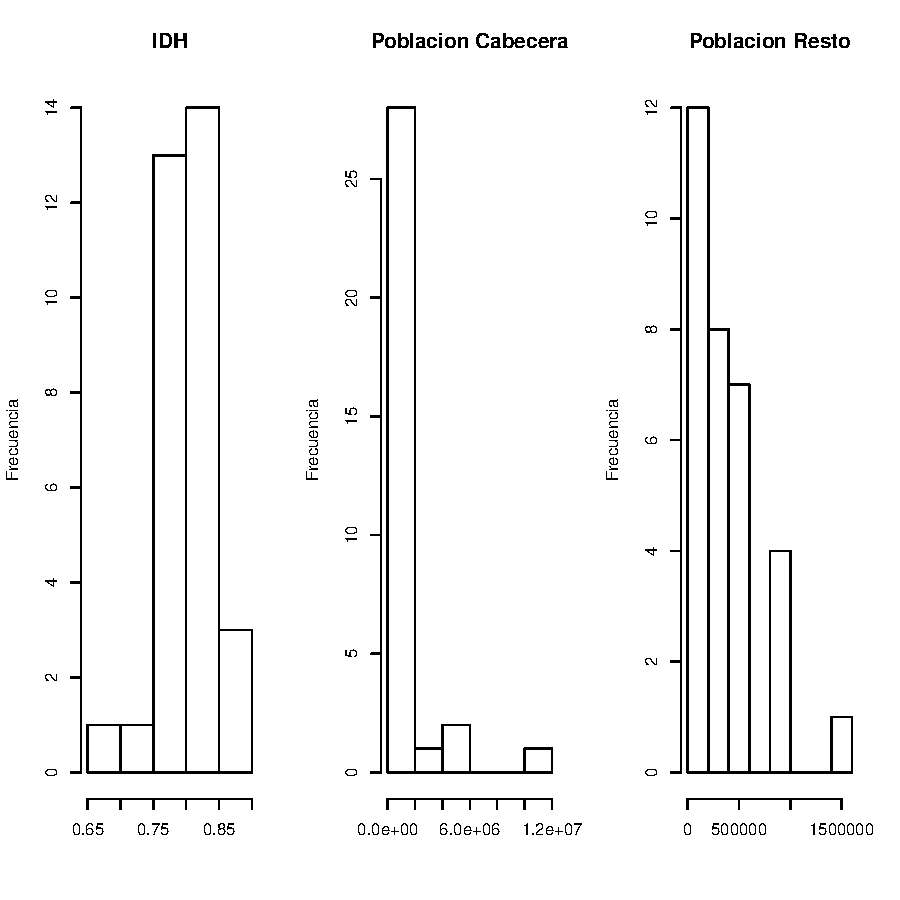
\includegraphics{ProyectoFInalLatex-barplots}
\end{adjustbox}
\caption{Histogramas IDH, Pobl. Cabecera y Pobl. Resto}
\label{barplots}
\end{figure}

Dado el sesgo de las poblaciones, podriamos transformarla para que se acerque a la realidad



%%%%% figure
\begin{figure}[h]
\centering
\begin{adjustbox}{width=10cm,height=6cm,trim=0cm 0.4cm 0cm 0cm}
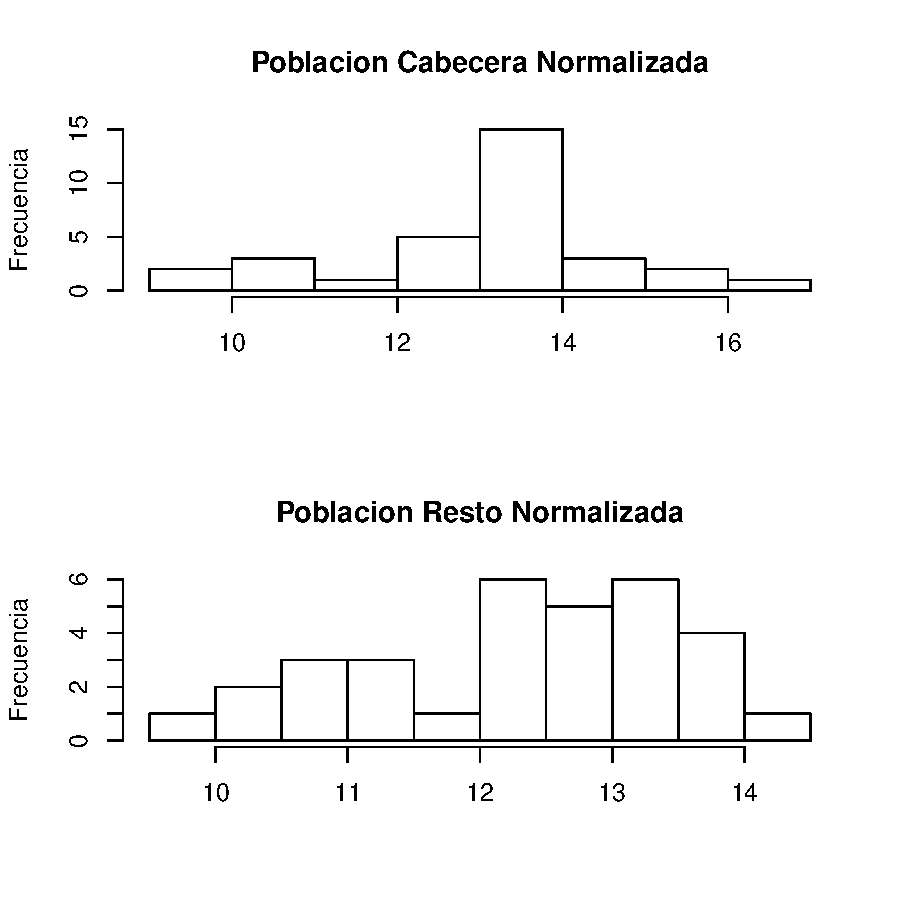
\includegraphics{ProyectoFInalLatex-barplots2}
\end{adjustbox}
\caption{Histogramas normalizados}
\label{barplots2}
\end{figure}
\clearpage

\section{Exploration Bivariada}\label{bivariada}
En esta seccion se vera la correlacion que tiene el IDH en relacion con las demas variables

En este trabajo estamos interesados en el impacto de la poblacion en el IDH, veamos IDH con cada uno:
% Table created by stargazer v.5.2.2 by Marek Hlavac, Harvard University. E-mail: hlavac at fas.harvard.edu
% Date and time: Sun, Jul 01, 2018 - 12:10:43
\begin{table}[!htbp] \centering 
  \caption{Correlacion del IDH con cada Poblacion} 
  \label{corrDem} 
\begin{tabular}{@{\extracolsep{5pt}} cc} 
\\[-1.8ex]\hline 
\hline \\[-1.8ex] 
PobCabeceraLog & PobRestoLog \\ 
\hline \\[-1.8ex] 
$0.487$ & $0.177$ \\ 
\hline \\[-1.8ex] 
\end{tabular} 
\end{table} 


Y la correlacion entre las variables independientes:



% Table created by stargazer v.5.2.2 by Marek Hlavac, Harvard University. E-mail: hlavac at fas.harvard.edu
% Date and time: Sun, Jul 01, 2018 - 12:10:43
\begin{table}[!htbp] \centering 
  \caption{Correlacion entre variables independientes} 
  \label{corrTableX} 
\begin{tabular}{@{\extracolsep{5pt}} ccc} 
\\[-1.8ex]\hline 
\hline \\[-1.8ex] 
 & PobCabeceraLog & PobRestoLog \\ 
\hline \\[-1.8ex] 
PobCabeceraLog & 1 &  \\ 
PobRestoLog & 0.84 & 1 \\ 
\hline \\[-1.8ex] 
\end{tabular} 
\end{table} 

Lo visto en la Tabla \ref{corrTableX} se refuerza claramente en la Figura \ref{corrPlotX}.
\begin{figure}[h]
\centering
\begin{adjustbox}{width=5cm,height=5cm}
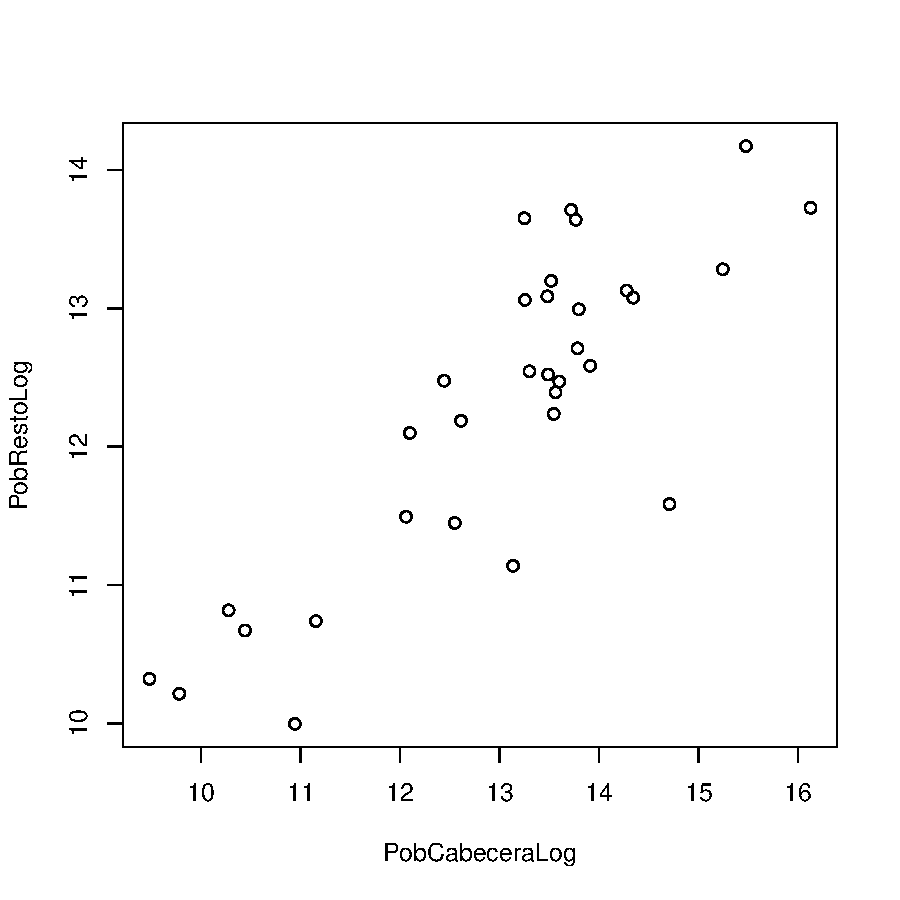
\includegraphics{ProyectoFInalLatex-corrPlotX}
\end{adjustbox}
\caption{correlacion entre las variables independientes}
\label{corrPlotX}
\end{figure}
\clearpage





\section{Modelos de Regresion}\label{regresion}

Veamos los modelos propuestos, primero sin poblacion resto, luego con esta:
% Table created by stargazer v.5.2.2 by Marek Hlavac, Harvard University. E-mail: hlavac at fas.harvard.edu
% Date and time: Sun, Jul 01, 2018 - 12:10:43
\begin{table}[!htbp] \centering 
  \caption{Modelos de Regresion} 
  \label{regresiones} 
\begin{tabular}{@{\extracolsep{5pt}}lcc} 
\\[-1.8ex]\hline 
\hline \\[-1.8ex] 
 & \multicolumn{2}{c}{\textit{Dependent variable:}} \\ 
\cline{2-3} 
\\[-1.8ex] & \multicolumn{2}{c}{IDH} \\ 
\\[-1.8ex] & (1) & (2)\\ 
\hline \\[-1.8ex] 
 PobCabeceraLog & 0.013$^{***}$ & 0.031$^{***}$ \\ 
  & (0.004) & (0.007) \\ 
  & & \\ 
 PobRestoLog &  & $-$0.030$^{***}$ \\ 
  &  & (0.010) \\ 
  & & \\ 
 Constant & 0.634$^{***}$ & 0.766$^{***}$ \\ 
  & (0.055) & (0.065) \\ 
  & & \\ 
\hline \\[-1.8ex] 
Observations & 32 & 32 \\ 
R$^{2}$ & 0.238 & 0.425 \\ 
Adjusted R$^{2}$ & 0.212 & 0.385 \\ 
Residual Std. Error & 0.037 (df = 30) & 0.033 (df = 29) \\ 
F Statistic & 9.347$^{***}$ (df = 1; 30) & 10.706$^{***}$ (df = 2; 29) \\ 
\hline 
\hline \\[-1.8ex] 
\textit{Note:}  & \multicolumn{2}{r}{$^{*}$p$<$0.1; $^{**}$p$<$0.05; $^{***}$p$<$0.01} \\ 
\end{tabular} 
\end{table} \clearpage

\section{Exploracion Espacial}\label{espacial}
Calculemos conglomerados de regiones,
usando toda la informaci??n de las tres variables.
usaremos la tecnica de k-means propuesta por MacQueen.




%%APLICANDO TECNICA KMEANS


\cite{macqueen_methods_nodate}

\begin{figure}[h]
\centering
%\begin{adjustbox}{width=11cm,height=8cm,clip,trim=1cm 2.5cm 0cm 2.5cm}
\begin{Schunk}
\begin{Soutput}
[1] 1 3 2
\end{Soutput}
\begin{Soutput}
  Group.1       IDH PobCabeceraLog PobRestoLog
1       1 0.7825714       10.58974    10.60684
2       2 0.7710833       13.28360    12.89513
3       3 0.8406154       14.12024    12.64415
\end{Soutput}
\end{Schunk}
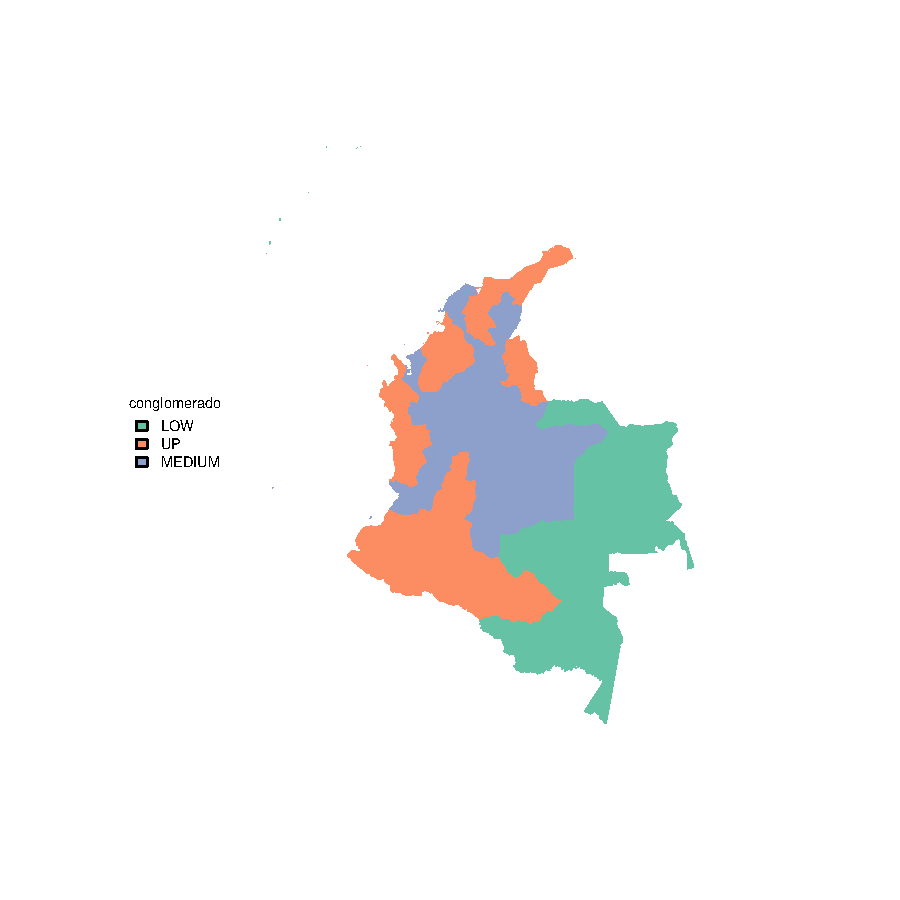
\includegraphics{ProyectoFInalLatex-plotMap}
%\end{adjustbox}
\caption{3 Clusters Departamentos de Colombia}\label{clustmap}
\end{figure}

\bibliographystyle{abbrv}
\renewcommand{\refname}{Bibliography}
\bibliography{Proyecto}

\end{document}
